\input{../YKY-preamble.tex}

\usepackage[backend=biber,bibstyle=authoryear,citestyle=../authoryearbrack]{biblatex}
\bibliography{../AGI-book}

\usepackage[CJKspace]{xeCJK}
\setCJKmainfont[BoldFont=SimHei,ItalicFont=KaiTi]{SimSun}
\usepackage{color}
\usepackage{mathtools}
\usepackage{hyperref}

\title{Co-operative genetic evolution of logic rules \\ {\normalsize white paper}}
% \author{general.intelligence@gmail.com}

\begin{document}
\maketitle

系统分为两部分:
\begin{itemize}
	\item 逻辑规则引擎 (logic rules engine)
	\item 基因算法 逻辑规则学习器 (genetic inductive learning of logic rules)
\end{itemize}

初步 测试 是「打井游戏」(tic-tac-toe),例如:
\begin{equation}
\begin{tabular}{c|c|c}
	$\bigcirc$ &          & $\times$ \\
\hline
	$\bigcirc$ & $\times$ & $\bigcirc$ \\
\hline
	           & $\times$ & $\bigcirc$ 
\end{tabular}
\end{equation}

\section{Genetic learning of rules}

\subsection{What is a logic rule?}

例如,数学式子可以表示成 tree, $V + F = E + 2$:
\begin{equation}
\vcenter{\hbox{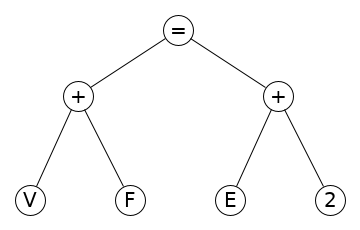
\includegraphics[scale=0.6]{Euler-formula.png}}}
\end{equation}

逻辑 rule 必然包含 $\Rightarrow$,可以将 rule 分成 \textbf{head} 和 \textbf{tail} 两部分:
\begin{equation}
\vcenter{\hbox{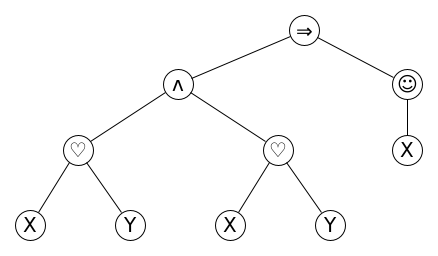
\includegraphics[scale=0.6]{I-love-you-n-you-love-me.png}}}
\end{equation}
\begin{equation}
\forall X, Y.  \quad \underbrace{X \heartsuit Y \wedge Y \heartsuit X}_{\mbox{head}} \Rightarrow \underbrace{\smiley X}_{\mbox{tail}}
\end{equation}

(这些可以在数学上严格定义,在论文中会详细定义)

Logic rule 的学习,即 inductive rule learning 又叫 inductive logic programming (ILP).  有基础的书介绍,例如:
\begin{equation}
\vcenter{\hbox{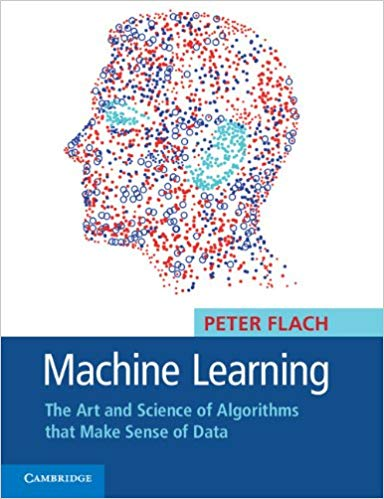
\includegraphics[scale=0.4]{Peter-Flach-machine-learning_COVER.jpg}}}
\quad \quad
\vcenter{\hbox{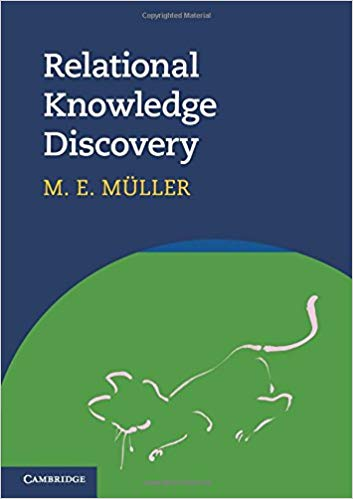
\includegraphics[scale=0.4]{relational-knowledge-discovery_COVER.jpg}}}
\end{equation}
可以上 \href{https://b-ok.org/}{https://b-ok.org/} 下载。  

Inductive logic learning 的参考书还有:
\begin{itemize}
	\item \citetitle{Raedt2008a} \parencite{Raedt2008a}
	\item \citetitle{Bergadano1996} \parencite{Bergadano1996}
	\item \citetitle{Lloyd2003} \parencite{Lloyd2003}
	\item \citetitle{Flach1994} \parencite{Flach1994}
	\item \citetitle{Fuernkranz2012} \parencite{Fuernkranz2012}
	\item \citetitle{Muggleton2015} \parencite{Muggleton2015}
	\item \citetitle{Raedt2016} \parencite{Raedt2016}
	\item \citetitle{Cussens2000} \parencite{Cussens2000}
	\item \citetitle{Dzeroski2001a} \parencite{Dzeroski2001a}
	\item \citetitle{Hitzler2011} \parencite{Hitzler2011}
\end{itemize}

这本身是一门颇深奥的学问,需要一段时间学习,但暂时不看也罢,只需要知道它是一种 combinatorial search,在 logic rules 的 lattice(格)中搜寻。 这是一种 离散的、符号的空间。

\subsection{Genetic algorithm}

要应用 GA 很容易,只需适当地 定义 cross-over 和 mutation.

\textbf{Cross-over}: 随机地选取一个节点,将两个式子在这点交叉。 

\textbf{Mutation}: 随机选择一个节点,在这个节点下换上一棵「随机树」(random tree)

\subsection{协同进化 (co-operative co-evolution)}

这部分是新的。 但它意思很明显,就是说: 进化的目标不只是一个最优的 个体,而是整个 群族。

The idea is first described in \parencite{Freitas2002}:
\begin{equation}
\vcenter{\hbox{\includegraphics[scale=2.0]{../../GILR/[Freitas]_quote_1.jpg}}}
\end{equation}

\begin{equation}
\vcenter{\hbox{\includegraphics[scale=0.5]{../../GILR/[Freitas]_quote_2.jpg}}}
\end{equation}

Two very early papers using genetic algorithm to learn logic rules are: \parencite{Giordana1994} and \parencite{Augier1995}.  There is also \parencite{Liu2000} which is an improvement over the SIA approach used in the above 2 papers.

\citetitle{Pietramala2008} \parencite{Pietramala2008} uses genetic algorithm to learn rules for document classification.  However, it uses only simple, propositional rules over $n$-grams.

One problem of genetic algorithms is that the genes represent \textbf{discrete} entities, so that crossing-over and mutations usually result in discrete \textbf{jumps} from one individual to another.  This is in contrast to deep learning where gradient descent is continuous.  Perhaps one way to circumvent this problem is to evolve a massive number of rules, and let the action of the intelligent agent be the \textbf{average} of a number of fired rules.  We will explore this idea.

\section{Logic rule engine}

其实这部分和 genetic algorithm 或 learning 都无关,但 logic rules 必需靠 逻辑引擎 运行 才能发生作用。 

逻辑 AI 引擎 的基本运作 如下:
\begin{equation}
\vcenter{\hbox{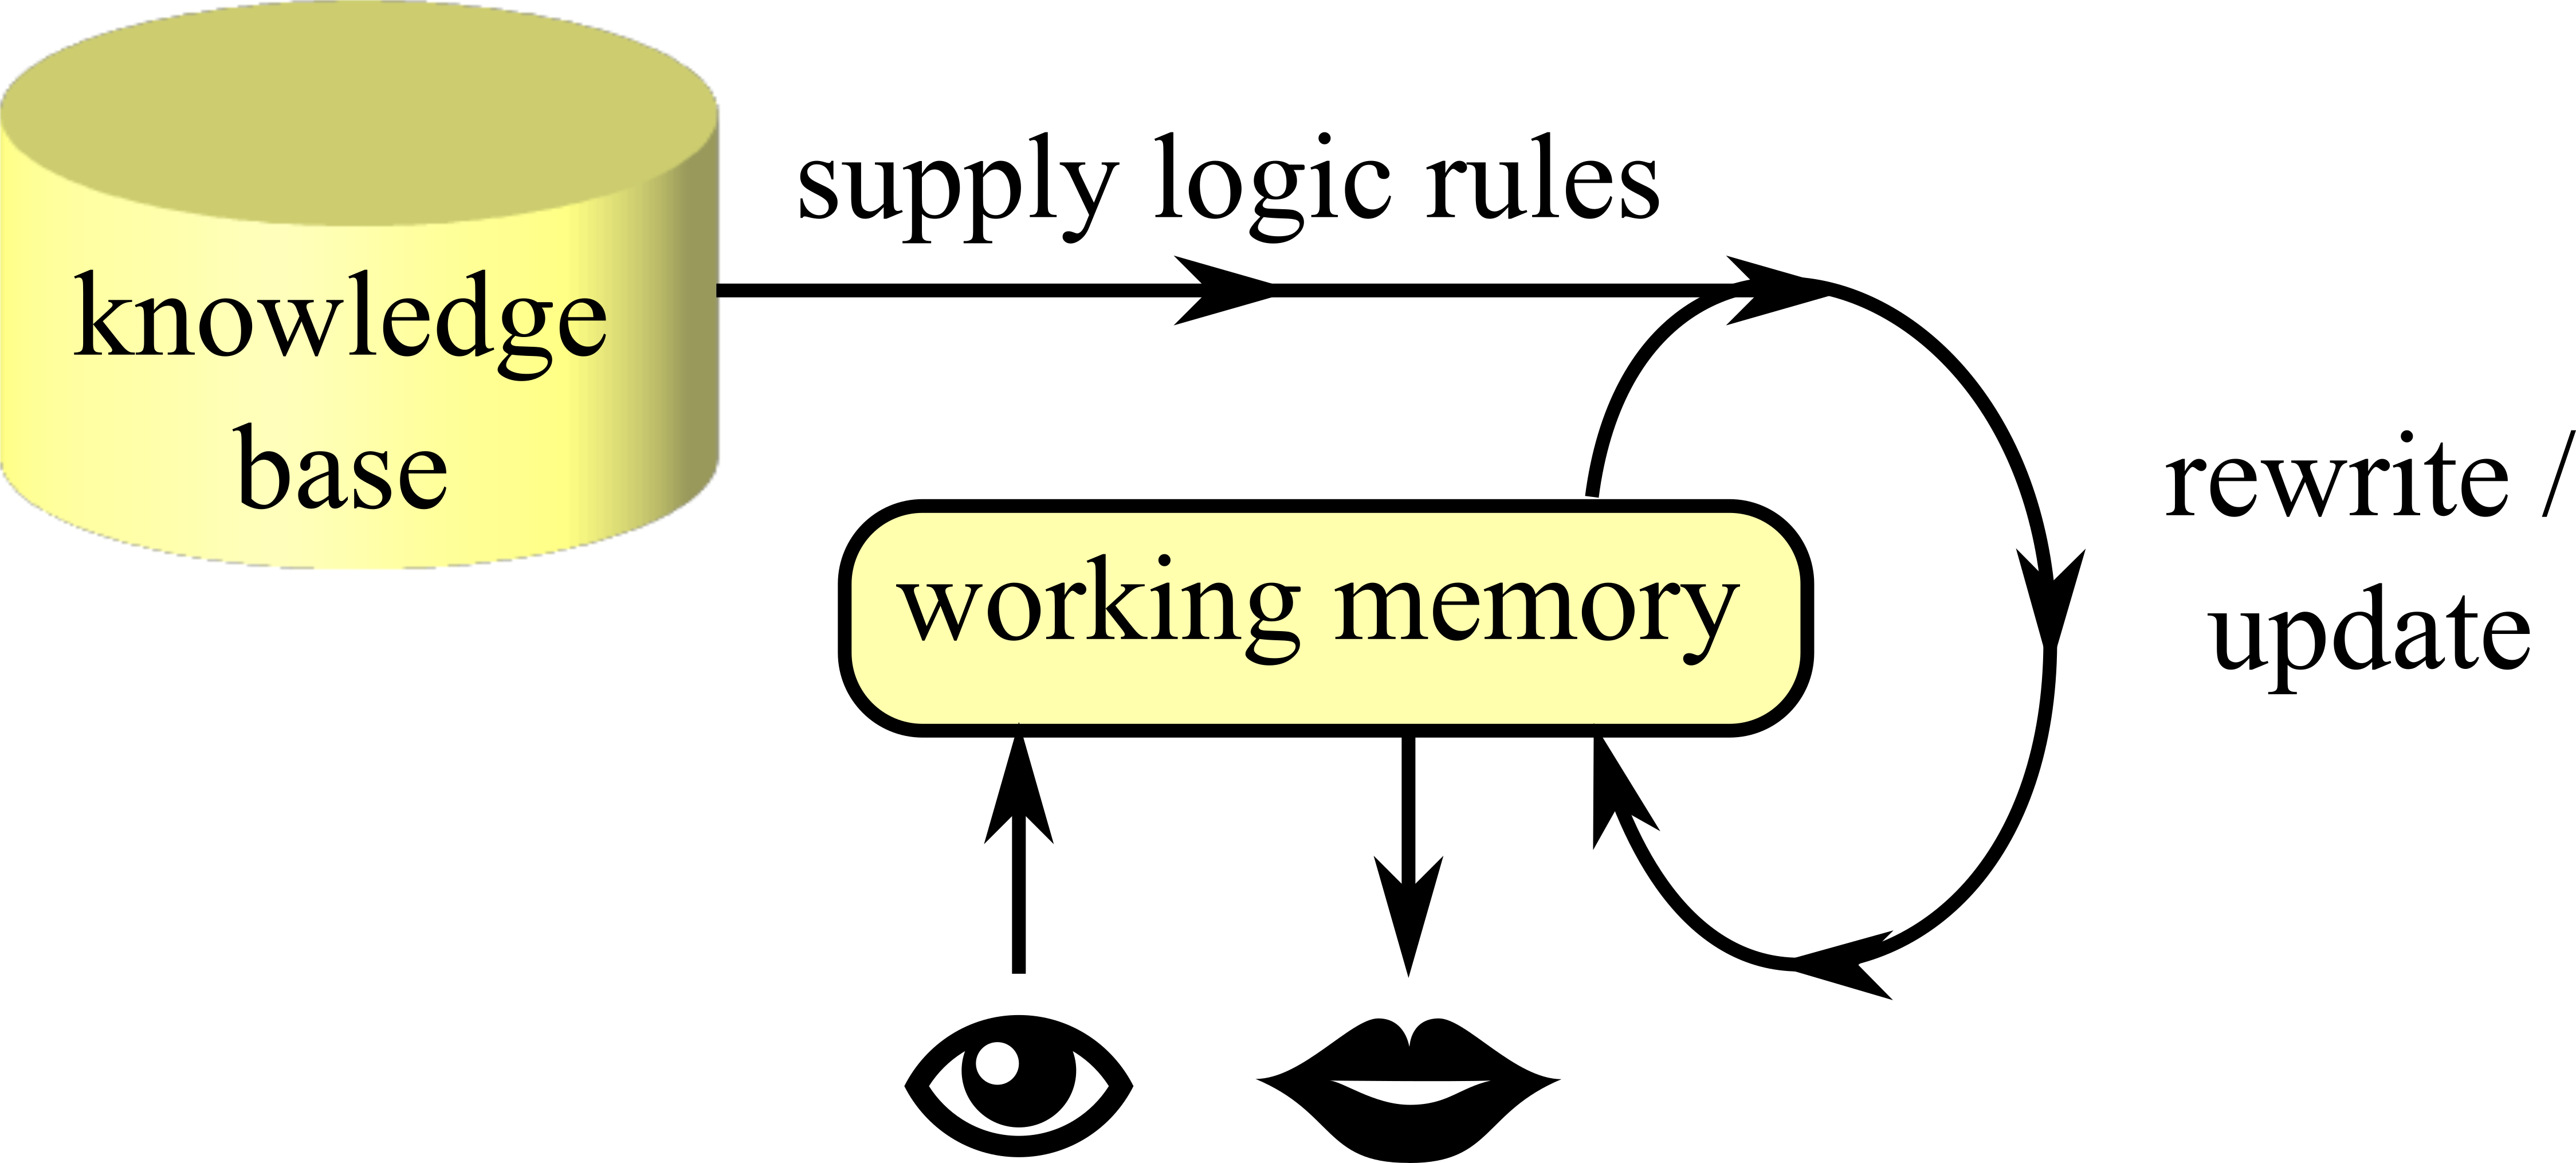
\includegraphics[scale=0.7]{LBAI-architecture.png}}}
\end{equation}

举例来说,例如打井游戏,游戏的 \textbf{状态} 是由一些 逻辑命题 描述: 
\begin{eqnarray}
	X(0,2) \nonumber \\
	X(1,1) \nonumber \\
	X(2,1) \nonumber \\
	O(0,0) \nonumber \\
	O(1,0) \nonumber \\
	O(1,2) \nonumber \\
	O(2,2) \nonumber \\
	\square(0,1) \nonumber \\
	\square(2,0)
\end{eqnarray}
表示这状态:
\begin{equation}
\begin{tabular}{c|c|c}
$\bigcirc$ &          & $\times$ \\
\hline
$\bigcirc$ & $\times$ & $\bigcirc$ \\
\hline
           & $\times$ & $\bigcirc$ 
\end{tabular}
\end{equation}

一条 logic rule 可以是这样:
\begin{equation}
\label{logic-rule-example}
X(x, y) \wedge X(w, y) \wedge \neq(x,w) \Rightarrow \text{ColumnWin}(x,y)
\end{equation}
表示如果有两个 X 在同一直行,则这一行差一步就可以赢。

其实我也不知道 打井游戏 的正确 rules 是怎样,这要等 learn 出来之后看看。 

在 (\ref{logic-rule-example}) 式里我用了 $\neq$ 这个 关系 (relation) 或 谓词 (predicate),其实是要额外定义的 (externally defined)。 详细来说这就像一种 programming language.

用读者的想像力脑补一下,可以明白到,这种逻辑引擎,基本上是可以解决任何问题的。 

\subsection{Rete algorithm}

(Rete 在 拉丁文的意思是「网状」)

其实这个算法也和学习无关,它只是 逻辑引擎 的一个 \textbf{加速} 算法,大部分 实际使用的逻辑引擎 都需要 Rete 的加速。

基本上,rete 算法将 logic rules 分拆、重组成 \textbf{树} 的结构:
\begin{equation}
\boxed{\text{logic rules}} \hookrightarrow \boxed{\text{树}} .
\end{equation}
这 tree 的意思和 decision tree 差不多。

逻辑引擎 运行时,从 input 输入一些 命题,进入 working memory.  这些 命题 传统上叫作 \textbf{WME} (working memory elements).  於是要将 WME 和 知识库中的 logic rules 逐一比较,看看哪条 rule 能够 apply,这过程称为 matching.  Rete 的作用是加速这 matching.

Rete 的 decision tree,输入是一个新的 WME,从树的 根 出发,比较有没有 match,如果有则记忆在树的节点里,如果没有则继续往下搜寻。

举个例: 「爱一个人但那人不爱你,则不开心」
\begin{equation}
\forall X, Y.  \quad \underbrace{X \heartsuit Y \wedge \neg Y \heartsuit X}_{\mbox{head}} \Rightarrow \underbrace{\frownie X}_{\mbox{tail}}
\end{equation}
在 rete 的树上会有节点检查 有没有 $\heartsuit$ 和 $\neg \heartsuit$ 这两个 WME,如果两个节点都通过,则有一链结会通往 结论的「激活」(fire). 

当然 rete 这个 tree 可以有不同的构造方法,类似 decision tree,例如根据 information gain. 

由於 rete 是树状结构,它是 hierarchical(层级化)的。 我们可以利用 rete 的层级化,将 进化算法 变成 层级化的。 这会是论文最大的贡献。

\section{Project status}

Our code is on GitHub: \\
\href{https://github.com/Cybernetic1/GILR}{https://github.com/Cybernetic1/GILR}

For the Rete algorithm, we adopted a simple open-source implementation called NaiveRete (written in Python) on GitHub.  NaiveRete is based on the PhD thesis of \cite{Doorenbos1995}.  When we fed randomly generated logic formulas into NaiveRete, we discovered some bugs and fixed them.

The Rete algorithm is notoriously difficult to understand and implement.  As a result, it is very difficult to conduct experiments in genetic learning of \textbf{first-order logic} formulas, which require an efficient logic engine to evaluate.  This may explain why this topic is relatively unexplored.

This is a Python example for setting up Rete and invoking it:
\begin{equation}
\vcenter{\hbox{\includegraphics[scale=0.6]{../../GILR/Genifer-lovers.png}}}
\end{equation}

The Rete network gets very big as more rules are added to it.  This is an example Rete network for only 1 rule:
\begin{equation}
\vcenter{\hbox{\includegraphics[scale=0.5]{../../GILR/rete_graph_ncc_test.png}}}
\end{equation}

This is a screenshot of the randomly generated logic rules for Tic-Tac-Toe:
\begin{equation}
\vcenter{\hbox{\includegraphics[scale=0.5]{../../GILR/logic_rules_screenshot.png}}}
\end{equation}

This is the GUI for the Tic-Tac-Toe learner:
\begin{equation}
\vcenter{\hbox{\includegraphics[scale=0.6]{../../GILR/GUI-screenshot.png}}}
\end{equation}

Currently the genetic algorithm fails to converge for Tic-Tac-Toe.  We think this is probably because the rules are ``flat'' in the sense that each rule looks at the board configuration and immediately concludes with a game move.  This class of rules may be inadequate for playing the game.  We think that adding \textbf{predicate invention} and \textbf{multi-step reasoning} would allow this game to be solved perfectly.

Then we will apply this algorithm on more challenging tasks such as natural language processing.

\printbibliography

\end{document}